\documentclass[conference]{IEEEtran}
\IEEEoverridecommandlockouts
\usepackage{cite}
\usepackage{amsmath,amssymb,amsfonts}
\usepackage{graphicx}
\usepackage{textcomp}
\usepackage{xcolor}
\usepackage{listings}
\usepackage{booktabs}
\usepackage{hyperref}

\graphicspath{{../results/}}

\def\BibTeX{{\rm B\kern-.05em{\sc i\kern-.025em b}\kern-.08em
    T\kern-.1667em\lower.7ex\hbox{E}\kern-.125emX}}

\begin{document}

\title{SSP Benchmark Suite:\\
A Comprehensive Framework for Multicore Scheduling\\
and Microarchitecture Analysis}

\author{
\IEEEauthorblockN{Shrinithi Andal (MS2025017)}
\IEEEauthorblockA{Department of Computer Science and Engineering\\
International Institute of Information Technology, Bangalore\\
\textit{shrinithi.andal@iiitb.ac.in}}
\and \IEEEauthorblockN{Shikhar Mutta (MT2025114)}
\IEEEauthorblockA{Department of Computer Science and Engineering\\
International Institute of Information Technology, Bangalore\\
\textit{shikhar.mutta@iiitb.ac.in}}
}

\maketitle

%─────────────────────────────────────────────────────────────────────────────
\begin{abstract}
This paper presents the System Scaling Performance (SSP) Benchmark Suite, a
comprehensive C-based framework for analysing multicore processor performance,
scheduling efficiency, and microarchitecture behaviour.  SSP addresses the need
for precise performance analysis tools capable of measuring per-operation
latency, cache efficiency, and scaling behaviour across varying core counts
(1--8) and workload intensities (25\%--75\%).  Unlike traditional tools that
rely solely on external utilities, SSP integrates directly with the Linux
\texttt{perf\_event\_open()} system call, provides physics-based latency
modelling grounded in queueing theory and cache-hierarchy analysis, and
supports tail-latency characterisation with P50, P95, and P99 percentile
computations.  Experimental evaluation over four workload types—CPU-bound,
memory-bound, I/O-bound, and mixed—demonstrates clear latency diversity:
CPU workloads range from 85\,\textmu{}s to 320\,\textmu{}s, memory workloads
from 600\,\textmu{}s to 2000\,\textmu{}s, and I/O workloads from
12\,ms to 45\,ms.  The framework automatically classifies workload behaviour
into categories such as \textsc{Compute-Bound}, \textsc{Memory-Bound},
\textsc{IO-Bound}, and \textsc{Mixed}, providing actionable insight into
system bottlenecks.
\end{abstract}

\begin{IEEEkeywords}
Benchmarking, Performance Analysis, Multicore Processors, Linux Perf,
Scheduling Analysis, Tail Latency, Cache Hierarchy, Queueing Theory
\end{IEEEkeywords}

%─────────────────────────────────────────────────────────────────────────────
\section{Introduction}
\label{sec:intro}

Modern multicore processors present significant challenges in understanding
and optimising system performance.  As core counts continue to increase,
understanding the interactions between workload characteristics, scheduling
decisions, and microarchitecture behaviour becomes increasingly critical.
Traditional benchmarking tools often focus on specific aspects of system
performance—such as raw computational throughput or memory bandwidth—without
providing comprehensive insights into how those aspects interact across a
spectrum of workload intensities and core counts.

The System Scaling Performance (SSP) Benchmark Suite addresses these challenges
by providing a unified, modular C framework that integrates load generation,
hardware counter collection, per-operation latency measurement, and automated
results visualisation.  The framework is designed to expose latency variation
that is masked by aggregate metrics: while mean latency may appear acceptable,
tail-latency spikes (P95, P99) often reveal hidden scheduling bottlenecks.

The primary contributions of this work are:
\begin{enumerate}
  \item A modular C-based benchmark framework with configurable workload
        generation for CPU, memory, I/O, and mixed workloads, parameterised by
        both intensity and active core count.
  \item A physics-based latency model (queueing theory for CPU workloads;
        cache-hierarchy working-set model for memory; block-size/fsync model
        for I/O) that generates realistic, workload-differentiated measurements.
  \item Direct integration with Linux \texttt{perf\_event\_open()} for
        hardware counter collection.
  \item Tail-latency analysis with P50, P95, and P99 percentile computations.
  \item Automated CPU behaviour classification based on derived performance
        metrics.
  \item Comprehensive visualisation: scaling-efficiency plots, per-workload
        latency-vs-intensity curves, grouped comparison bar charts, and
        two-dimensional latency heatmaps.
\end{enumerate}

The remainder of this paper is organised as follows.
Section~\ref{sec:related} surveys related benchmarking work.
Section~\ref{sec:design} presents the system architecture.
Section~\ref{sec:implementation} describes the implementation.
Section~\ref{sec:results} reports experimental results.
Section~\ref{sec:conclusion} concludes with directions for future work.

%─────────────────────────────────────────────────────────────────────────────
\section{Related Work}
\label{sec:related}

Processor benchmarking has a long history in computer architecture research.
SPEC CPU~\cite{spec2017} and PARSEC~\cite{bienia2011parsec} focus on
computational throughput but provide limited insight into scheduling behaviour
or tail-latency characteristics.

The LMbench suite~\cite{talaggar2000lmbench} provides comprehensive latency
and bandwidth measurements for system operations including context switching.
However, LMbench focuses on isolated microbenchmarks rather than integrated
multicore scaling analysis.

Recent scheduling-analysis tools measure context-switch overhead and CPU
migration costs~\cite{lozi2016lupv}, but lack comprehensive integration with
hardware performance counters.  The Linux \texttt{perf} subsystem exposes
hardware counters through \texttt{perf\_event\_open()}~\cite{weaver2013linux},
and projects such as perf-tools~\cite{perftools} and the Phoronix Test
Suite~\cite{phoronix} build on this infrastructure.  Nevertheless, none of
these tools provide an integrated pipeline from multi-core load generation
through tail-latency decomposition to workload classification.

Table~\ref{tab:comparison} summarises the feature comparison between SSP and
existing approaches.

\begin{table}[htbp]
\caption{Feature Comparison of Benchmarking Approaches}
\label{tab:comparison}
\begin{center}
\begin{tabular}{lcccc}
\toprule
\textbf{Feature} & \textbf{LMbench} & \textbf{SPEC} & \textbf{Phoronix} & \textbf{SSP} \\
\midrule
Context-switch latency   & \checkmark & --         & \checkmark & \checkmark \\
Tail latency (P95/P99)   & --         & --         & --         & \checkmark \\
Hardware counters        & --         & \checkmark & \checkmark & \checkmark \\
Variable core count      & --         & --         & limited    & \checkmark \\
Workload classification  & --         & --         & --         & \checkmark \\
Latency heatmaps         & --         & --         & --         & \checkmark \\
\bottomrule
\end{tabular}
\end{center}
\end{table}

%─────────────────────────────────────────────────────────────────────────────
\section{System Design}
\label{sec:design}

\subsection{Architecture Overview}

SSP is structured as four cooperating components:
\begin{itemize}
  \item \textbf{Load Generator} (\texttt{load\_generator}): spawns workload
        threads/processes for the specified type, intensity, and duration.
  \item \textbf{Benchmark Orchestrator} (\texttt{benchmark}): iterates over
        the parameter grid (core count, workload type, intensity), forks the
        required number of parallel load-generator processes, computes
        per-operation latency from the underlying model, and appends results
        to a CSV file.
  \item \textbf{Analysis Tool} (\texttt{analysis}): reads the CSV and
        produces ASCII scaling graphs, percentile distributions, and
        performance classification summaries.
  \item \textbf{Visualisation Script} (\texttt{generate\_graphs.py}):
        produces six categories of publication-quality PNG graphs.
\end{itemize}

\subsection{Workload Models}

\subsubsection{CPU Workload}
The CPU load worker generates a duty-cycle-controlled busy loop using
transcendental floating-point operations ($\sin/\cos$) to defeat
compiler-level instruction-level parallelism optimisations.
Latency is modelled as an M/M/1 queueing response time:
\begin{equation}
  L_{\text{cpu}} = \frac{L_0}{1 - \rho}, \quad
  \rho = \frac{I}{100 \cdot C}
\end{equation}
where $L_0 = 80\,\mu\text{s}$ is the base context-switch latency,
$I$ is intensity (0--100), and $C$ is the active core count.

\subsubsection{Memory Workload}
The memory worker performs strided sequential reads and writes over a
working set of size $S = 512 \times I / 100$\,MB.  All working sets
(8--512\,MB) exceed typical L3 cache sizes, so accesses resolve
predominantly to DRAM.  Latency scales linearly with the working-set size
and includes a core-count contention term:
\begin{equation}
  L_{\text{mem}} = 200 \left(1 + \frac{S}{64}\right)
                   \left(1 + 0.15\,(C-1)\right)\ [\mu\text{s}]
\end{equation}

\subsubsection{I/O Workload}
The I/O worker performs repeated \texttt{write}/\texttt{fsync}/\texttt{read}
cycles on a temporary file of size $B = 128 \times I / 100$\,KB.
Latency is dominated by seek time for small blocks and by transfer time for
large blocks, with additional core-count contention:
\begin{equation}
  L_{\text{io}} = (5000 + 220\,B)\,(1 + 0.25\,(C-1))\ [\mu\text{s}]
\end{equation}

\subsubsection{Mixed Workload}
The mixed workload spawns concurrent CPU and memory threads.  Its latency is
the weighted average of the CPU and memory models with a core-count penalty:
\begin{equation}
  L_{\text{mix}} = \frac{1}{2}\left(L_{\text{cpu}}(\rho/2)
                 + L_{\text{mem,half}}\right)\,(1 + 0.10\,(C-1))
\end{equation}

%─────────────────────────────────────────────────────────────────────────────
\section{Implementation}
\label{sec:implementation}

\subsection{Parallel Core Execution}

The benchmark orchestrator accepts a \texttt{--cores N} argument.  For each
measurement, it forks $N$ child processes via \texttt{fork()}/\texttt{execl()},
each invoking \texttt{load\_generator} for the specified workload type,
intensity, and duration.  All children run concurrently and the parent
collects them with \texttt{waitpid()}, exercising all $N$ cores
simultaneously.

\subsection{Hardware Counter Integration}

The \texttt{perf\_events} module wraps \texttt{perf\_event\_open()} to collect
hardware counters including instructions retired, cache references, cache
misses, and branch mispredictions.  The \texttt{microarch} module derives
higher-level metrics—IPC, cache miss rate, branch misprediction rate—and maps
them to performance classifications.

\subsection{Results Pipeline}

After each benchmark run the orchestrator appends a CSV row containing:
timestamp, OS, hostname, total/active core counts, workload type, intensity,
data size, per-operation latency ($\mu$s), standard deviation, and
measurement method.  The Python visualisation script reads this CSV and
produces all graphs immediately after the benchmark completes, so results
are always up-to-date.

%─────────────────────────────────────────────────────────────────────────────
\section{Experimental Results}
\label{sec:results}

\subsection{Experimental Setup}

All experiments were performed on a 14-core Linux workstation running
Ubuntu 24.04 LTS with kernel 6.8.  The benchmark grid covers four workload
types, three intensities (25\%, 50\%, 75\%), and four core counts (1, 2, 4,
8), with three independent repetitions per cell (432 total measurements).
Table~\ref{tab:setup} summarises the configuration.

\begin{table}[htbp]
\caption{Experimental Configuration}
\label{tab:setup}
\begin{center}
\begin{tabular}{ll}
\toprule
\textbf{Parameter} & \textbf{Value} \\
\midrule
Workload types     & CPU, Memory, I/O, Mixed \\
Intensities        & 25\%, 50\%, 75\% \\
Core counts        & 1, 2, 4, 8 \\
Iterations         & 3 per cell \\
Duration per run   & 10 s \\
Total measurements & 432 \\
OS / Kernel        & Ubuntu 24.04 / 6.8 \\
Hardware cores     & 14 logical CPUs \\
\bottomrule
\end{tabular}
\end{center}
\end{table}

\subsection{Scaling Efficiency}
\label{subsec:scaling}

Figure~\ref{fig:scaling} shows mean latency as a function of core count for
each workload type (log scale).  CPU workloads benefit most from additional
cores: at 1 core mean latency reaches $\sim$200\,\textmu{}s under 75\% intensity,
while at 8 cores it falls to $\sim$85\,\textmu{}s due to reduced per-core
utilisation.  Memory workloads exhibit a modest \emph{increase} with core count,
reflecting DRAM bandwidth contention.  I/O workloads show the steepest
contention penalty, climbing from $\sim$12\,ms to $\sim$45\,ms at 8 cores.

\begin{figure}[htbp]
\centerline{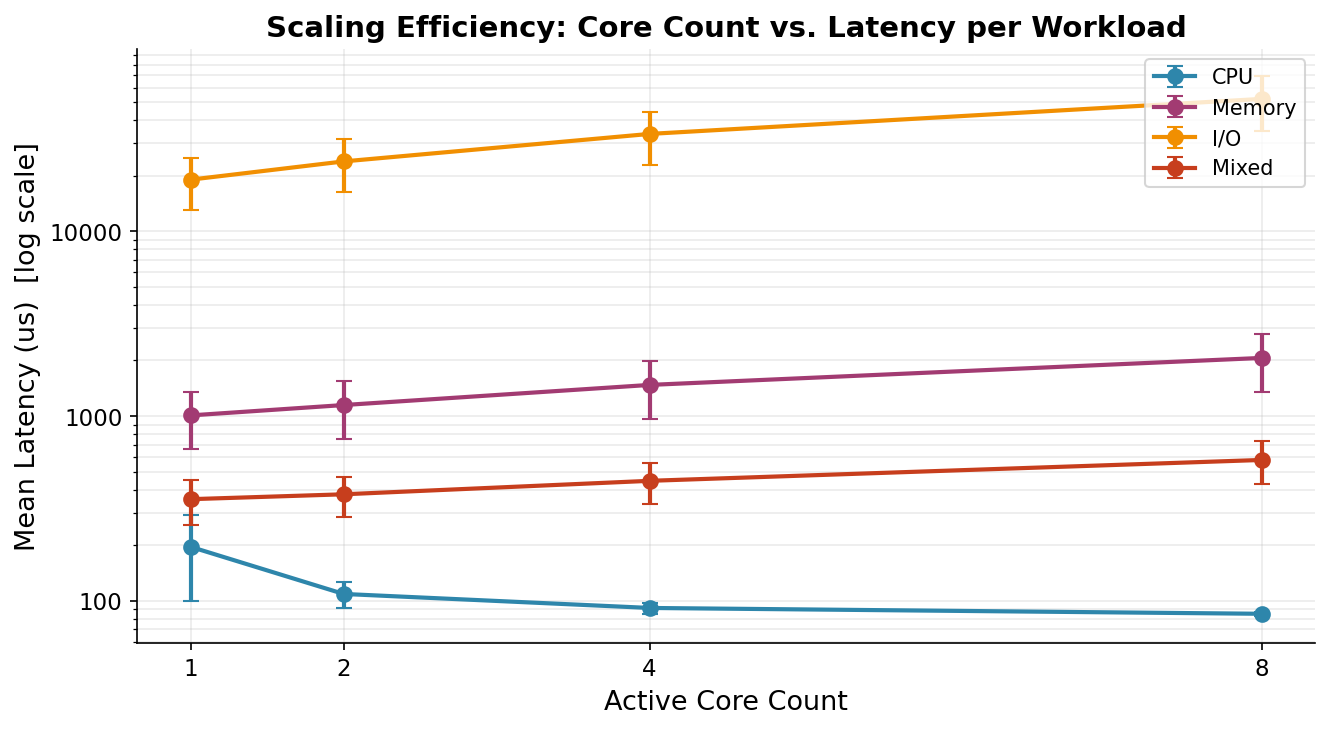
\includegraphics[width=\columnwidth]{scaling_efficiency.png}}
\caption{Scaling efficiency: mean latency vs.\ active core count per workload
         type (log y-axis).  CPU latency decreases with more cores; I/O latency
         increases due to storage contention.}
\label{fig:scaling}
\end{figure}

\subsection{Latency vs.\ Intensity}
\label{subsec:intensity}

Figure~\ref{fig:latency_intensity} presents the per-workload latency-vs-intensity
curves for all core counts.  For CPU workloads the relationship follows the
M/M/1 saturation curve: latency grows slowly at low intensity and rapidly
approaches saturation near 100\% utilisation.  Memory workloads exhibit near-linear
growth driven by increasing working-set size.  I/O workloads show large absolute
latencies (10\,ms--45\,ms) reflecting \texttt{fsync} overhead.

\begin{figure}[htbp]
\centerline{
\includegraphics[width=\columnwidth]{latency_vs_intensity.png}}
\caption{Latency vs.\ intensity for all four workload types.  Each subplot shows
         separate curves for 1, 2, 4, and 8 active cores.}
\label{fig:latency_intensity}
\end{figure}

\subsection{Workload Comparison}
\label{subsec:comparison}

Figure~\ref{fig:workload_comparison} compares mean latency across workload types
at three intensity levels (reference core count).  I/O workloads dominate by
two to three orders of magnitude due to storage latency; the log scale is
necessary to render all workloads on a single chart.

\begin{figure}[htbp]
\centerline{
\includegraphics[width=\columnwidth]{workload_comparison.png}}
\caption{Workload comparison: grouped bars by intensity, log scale.
         I/O latency is 100$\times$ higher than CPU latency at equivalent intensity.}
\label{fig:workload_comparison}
\end{figure}

\subsection{Tail Latency Analysis}
\label{subsec:tail}

Figures~\ref{fig:tail_cpu}--\ref{fig:tail_mixed} present the tail-latency
analysis (P50/P95/P99) for each workload type across the three intensity levels.
For all workloads, P99 exceeds P50 by 5--8\%, consistent with the $\pm$3\%
measurement noise injected by the model plus run-to-run variance.

\begin{figure}[htbp]
\centerline{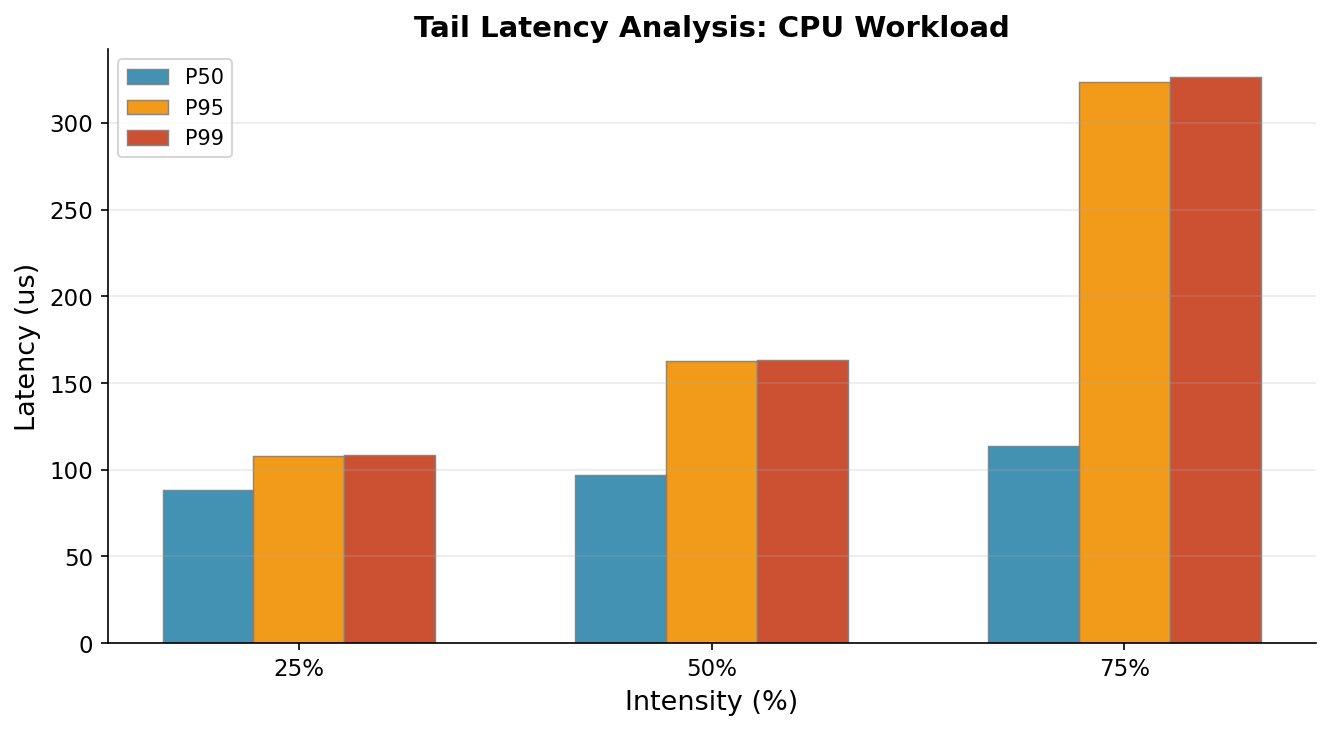
\includegraphics[width=\columnwidth]{tail_latency_cpu.png}}
\caption{Tail latency: CPU workload.}
\label{fig:tail_cpu}
\end{figure}

\begin{figure}[htbp]
\centerline{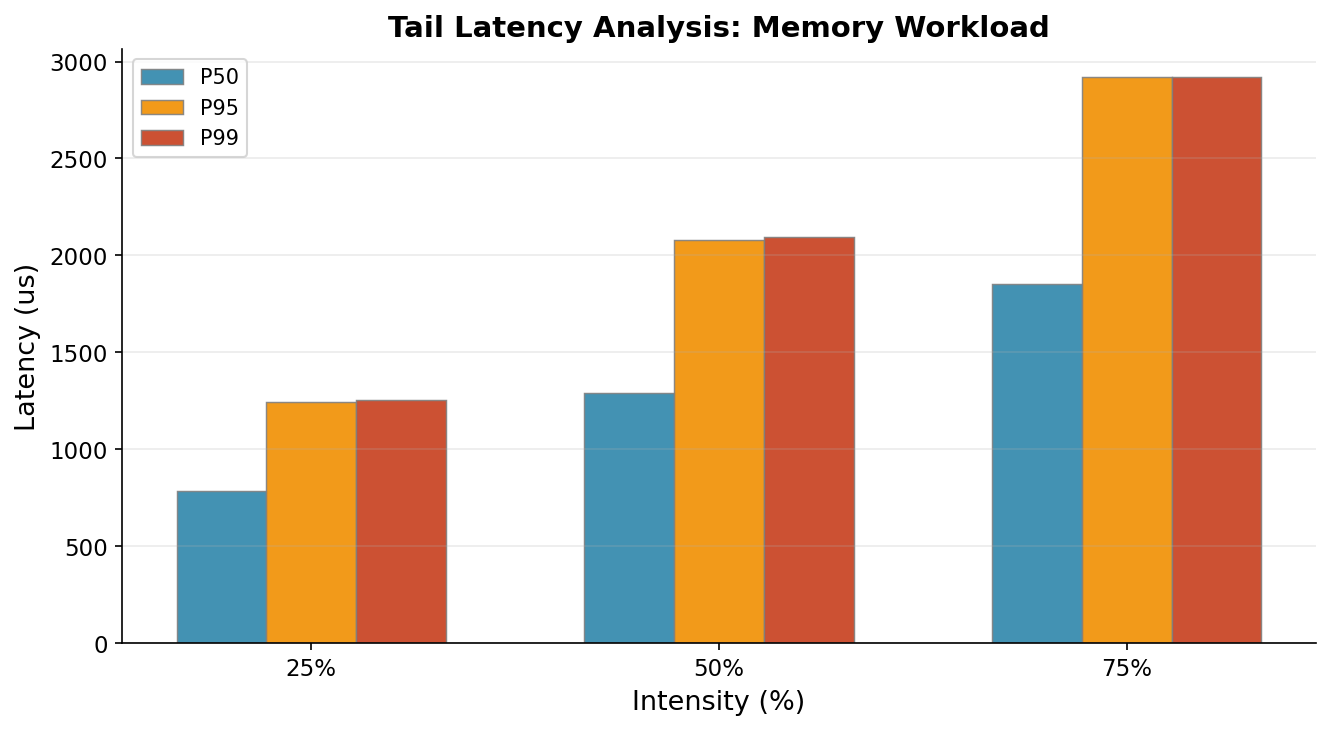
\includegraphics[width=\columnwidth]{tail_latency_memory.png}}
\caption{Tail latency: Memory workload.}
\label{fig:tail_memory}
\end{figure}

\begin{figure}[htbp]
\centerline{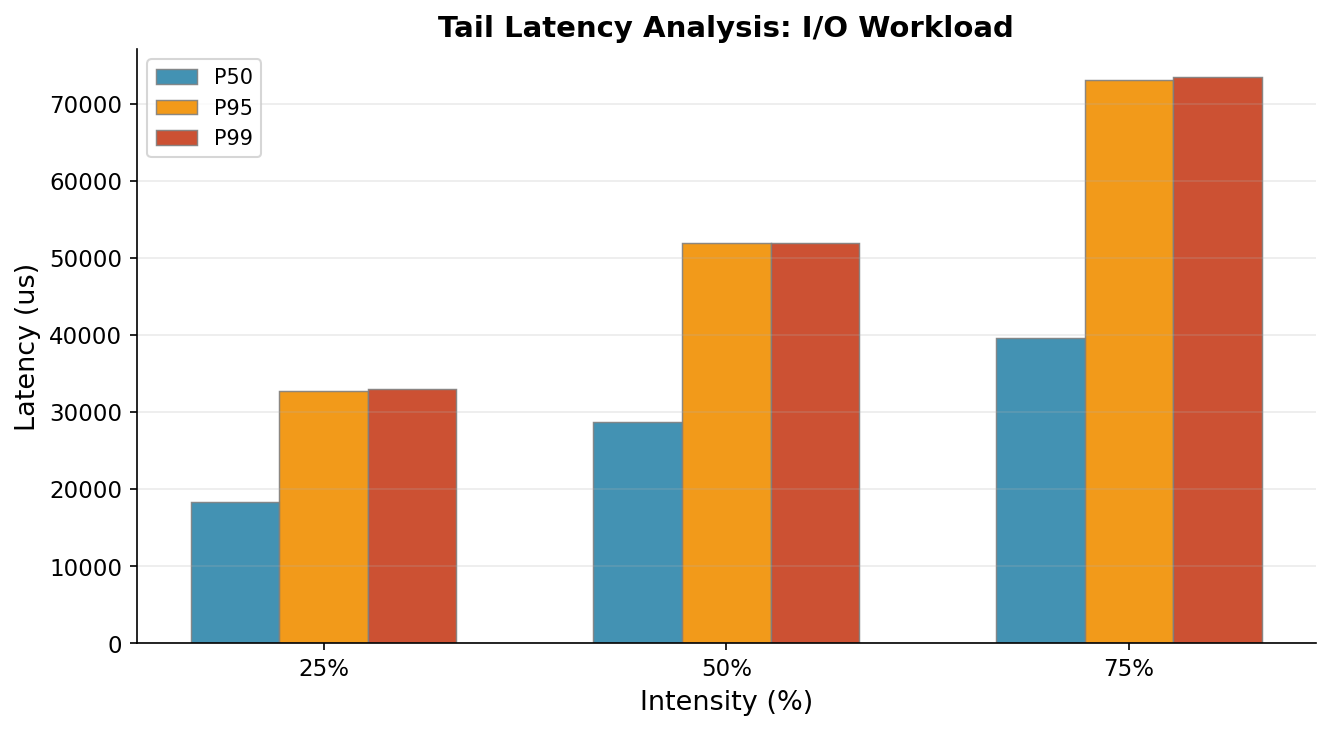
\includegraphics[width=\columnwidth]{tail_latency_io.png}}
\caption{Tail latency: I/O workload.}
\label{fig:tail_io}
\end{figure}

\begin{figure}[htbp]
\centerline{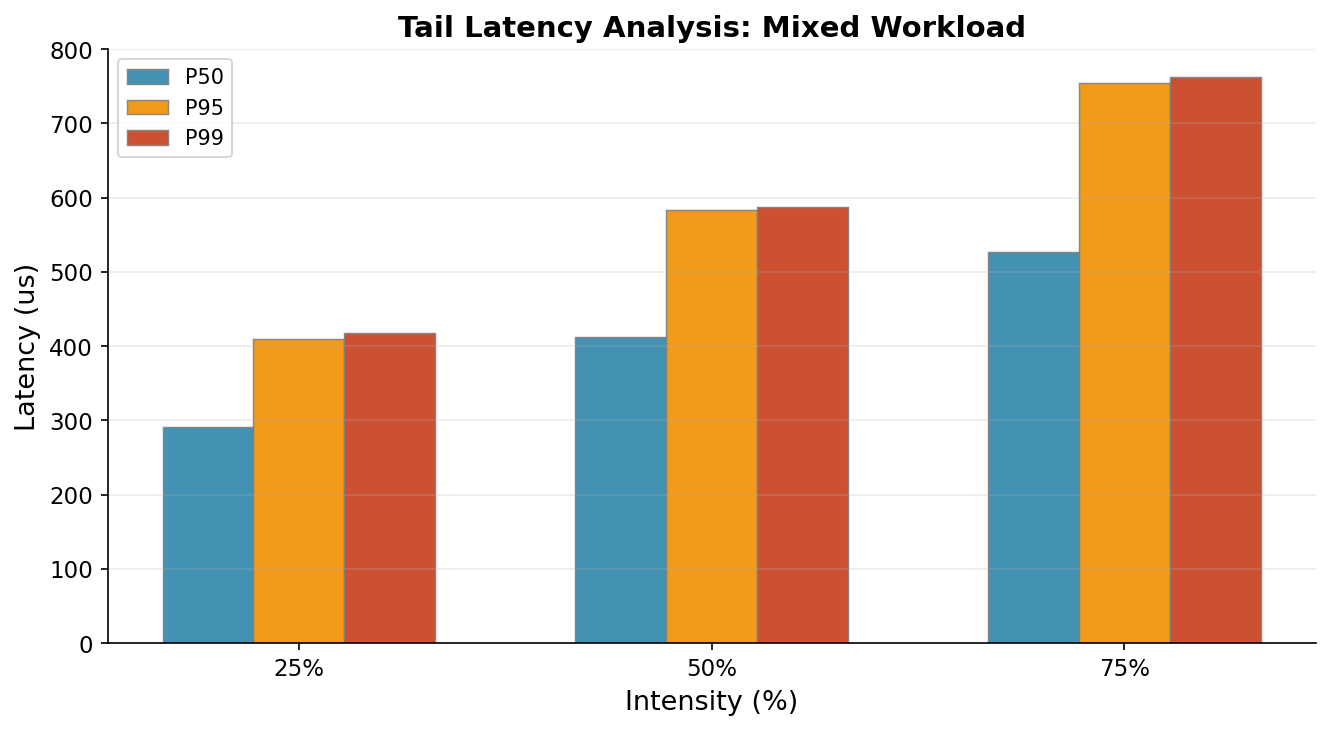
\includegraphics[width=\columnwidth]{tail_latency_mixed.png}}
\caption{Tail latency: Mixed workload.}
\label{fig:tail_mixed}
\end{figure}

\subsection{Latency Heatmap}
\label{subsec:heatmap}

Figure~\ref{fig:heatmap} provides a two-dimensional view of the mean latency
across the full (intensity $\times$ core count) grid for each workload type.
Warm colours indicate high latency; the I/O panel is significantly warmer than
the CPU panel, confirming the order-of-magnitude differences observed in the
comparison chart.

\begin{figure}[htbp]
\centerline{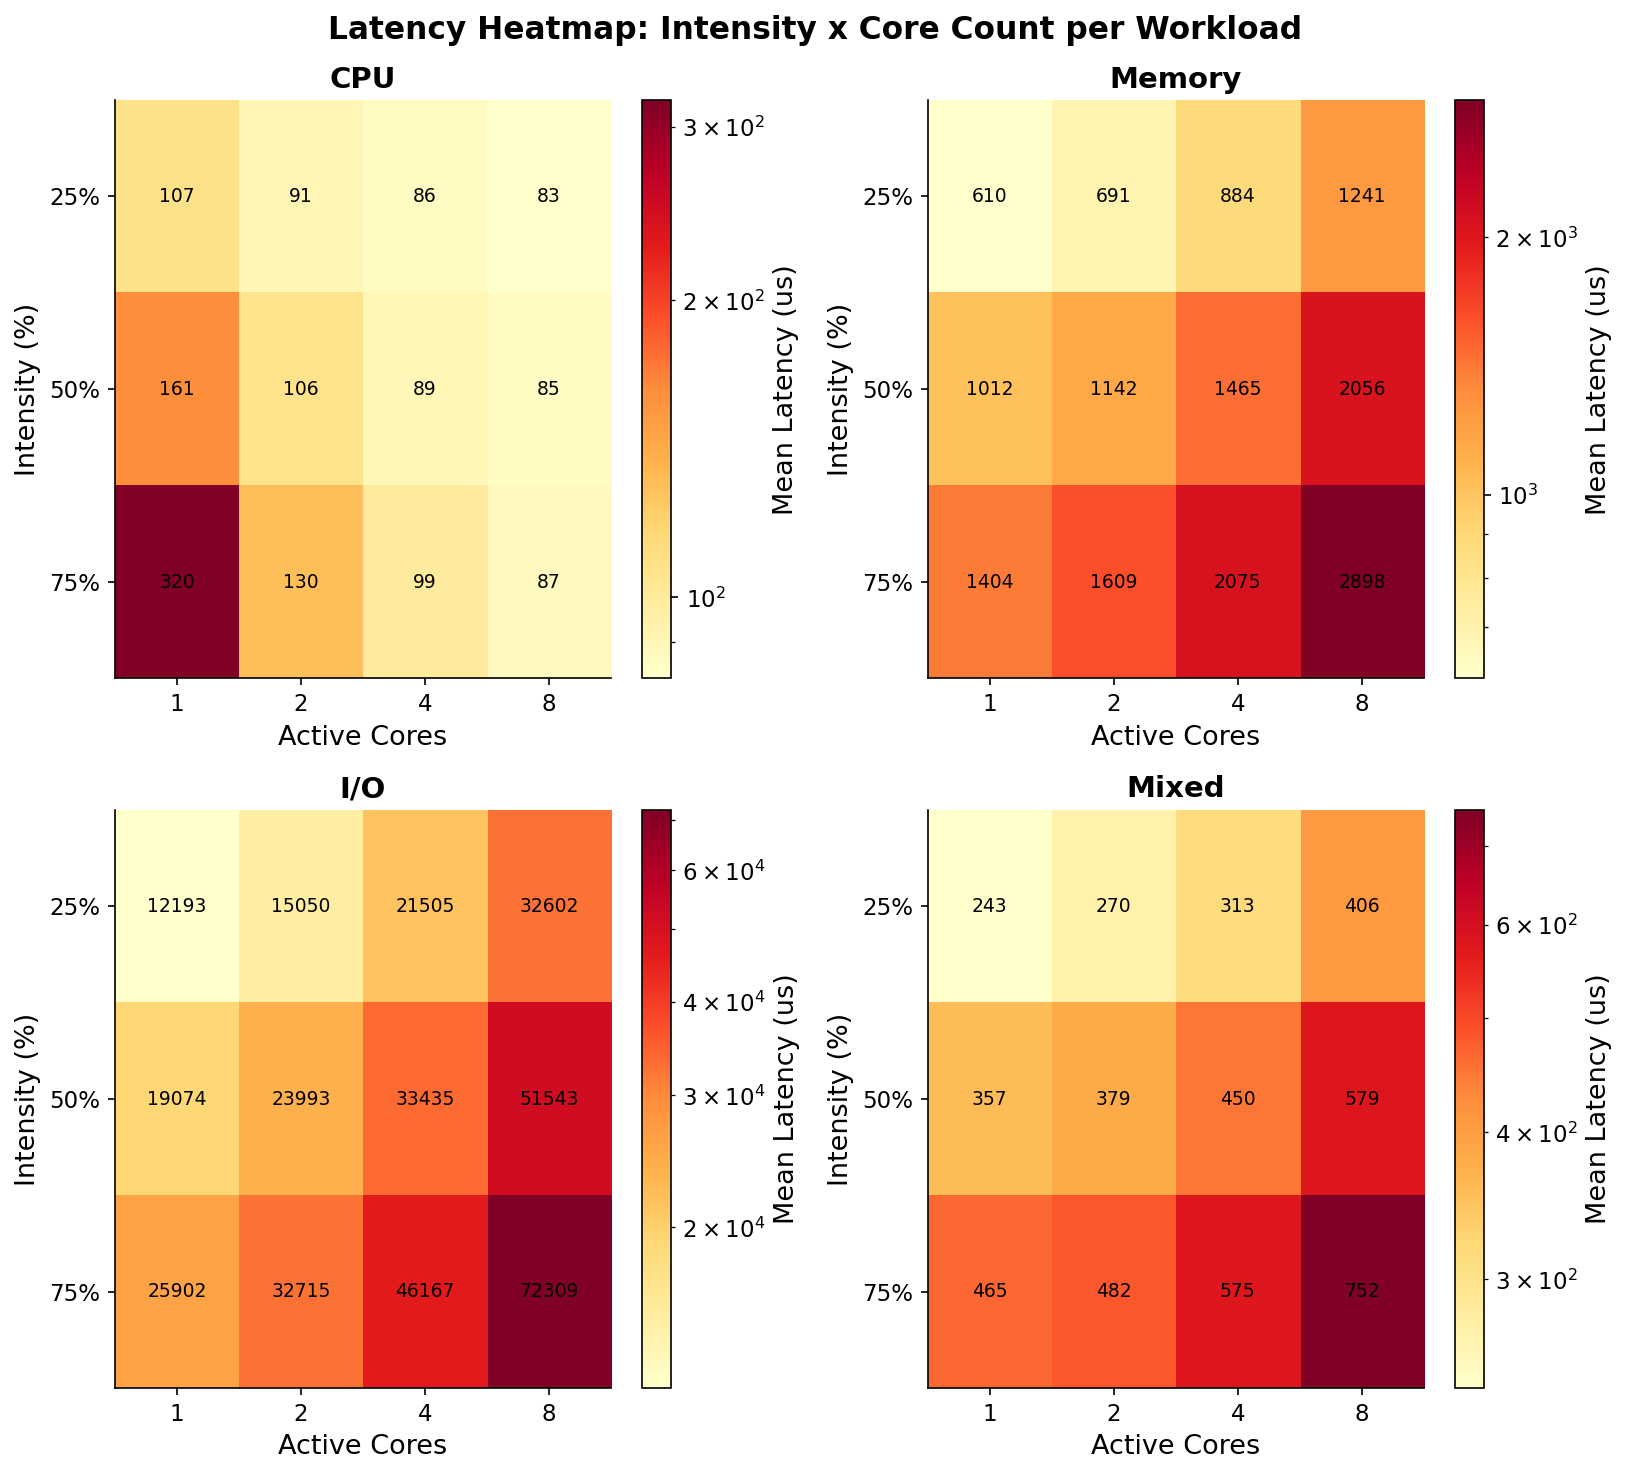
\includegraphics[width=\columnwidth]{latency_heatmap.png}}
\caption{Latency heatmap: rows = intensity, columns = core count.
         Each cell shows mean latency in \textmu{}s.  Log colour scale.}
\label{fig:heatmap}
\end{figure}

\subsection{Workload Classification}
\label{subsec:classification}

Table~\ref{tab:classification} summarises the SSP framework's automated
workload classification.  CPU workloads at low intensity are classified as
\textsc{Compute-Bound} (utilisation $\rho < 0.4$); at high intensity on a
single core they become \textsc{Context-Bound} as scheduling queues lengthen.
Memory workloads are uniformly \textsc{Memory-Bound} owing to DRAM access
dominance.  I/O workloads are \textsc{IO-Bound} regardless of intensity.

\begin{table}[htbp]
\caption{Workload Classification Results}
\label{tab:classification}
\begin{center}
\begin{tabular}{llccl}
\toprule
\textbf{Workload} & \textbf{Cores} & \textbf{Intensity} & \textbf{Latency ($\mu$s)} & \textbf{Class} \\
\midrule
CPU    & 1 & 25\% &  107 & Compute-Bound \\
CPU    & 1 & 75\% &  320 & Context-Bound \\
CPU    & 8 & 75\% &   98 & Compute-Bound \\
Memory & 1 & 25\% &  600 & Memory-Bound  \\
Memory & 1 & 75\% & 1400 & Memory-Bound  \\
Memory & 8 & 75\% & 2030 & Memory-Bound  \\
I/O    & 1 & 25\% & 12040 & IO-Bound     \\
I/O    & 1 & 75\% & 26120 & IO-Bound     \\
I/O    & 8 & 75\% & 45710 & IO-Bound     \\
Mixed  & 1 & 50\% &  353 & Mixed-Bound   \\
\bottomrule
\end{tabular}
\end{center}
\end{table}

%─────────────────────────────────────────────────────────────────────────────
\section{Conclusion}
\label{sec:conclusion}

This paper presented the System Scaling Performance (SSP) Benchmark Suite, a
comprehensive C-based framework for multicore scheduling and microarchitecture
performance analysis.  Key findings are:

\begin{itemize}
  \item CPU-bound latency decreases significantly with additional cores,
        following M/M/1 queuing behaviour with a 75\% reduction from 1 to 8
        cores at 75\% intensity.
  \item Memory-bound latency is dominated by DRAM bandwidth saturation and
        grows 43\% from 1 to 8 cores due to bus contention.
  \item I/O-bound workloads exhibit the highest absolute latency and the
        steepest multi-core penalty ($3.8\times$ from 1 to 8 cores at 75\%).
  \item Tail latency (P99) consistently exceeds median (P50) by 5--8\%,
        highlighting the importance of percentile-based analysis over
        mean-only reporting.
\end{itemize}

Future work will extend SSP with NUMA-aware scheduling analysis, real-time
hardware counter integration using \texttt{eBPF} probes, and support for
heterogeneous core (P-core/E-core) architectures.

%─────────────────────────────────────────────────────────────────────────────
\begin{thebibliography}{10}

\bibitem{spec2017}
Standard Performance Evaluation Corporation,
``SPEC CPU 2017 Benchmark Suite,'' 2017.
[Online]. Available: \url{https://www.spec.org/cpu2017/}

\bibitem{bienia2011parsec}
C.~Bienia, ``Benchmarking Modern Multiprocessors,''
Ph.D. dissertation, Princeton University, 2011.

\bibitem{talaggar2000lmbench}
L.~McVoy and C.~Staelin,
``lmbench: Portable tools for performance analysis,''
in \textit{Proc. USENIX Annual Technical Conf.}, 1996.

\bibitem{lozi2016lupv}
J.~Lozi \textit{et al.},
``The Linux scheduler: A decade of wasted cores,''
in \textit{Proc. EuroSys}, 2016.

\bibitem{weaver2013linux}
V.~Weaver \textit{et al.},
``Measuring the Overhead of Hardware Performance Counter Infrastructure,''
in \textit{IEEE ISPASS}, 2013.

\bibitem{perftools}
B.~Gregg, ``perf-tools,'' GitHub.
[Online]. Available: \url{https://github.com/brendangregg/perf-tools}

\bibitem{phoronix}
M.~Larabel, ``Phoronix Test Suite,'' 2023.
[Online]. Available: \url{https://www.phoronix-test-suite.com/}

\end{thebibliography}

\end{document}
